\section{Objectives Summarised}

    \begin{enumerate}
        \item The program should be capable of procedurally drawing a road network to the UI using point vertices and cubic Bezier curves to model roads.
        \item The number of vertices should be limited to 50 to prevent slowing down the simulation.
        \item The user should be able to save and load road networks in and out of the program.
        \item The program should support a click-and-drag based interaction, allowing the creation of vertices and connections and further editing of the network.
        \item The user should also be able to undo and redo actions to the road network.
        \item The program should be able to simulate cars driving sensibly across the road network.
        \item The maximum number of agents active at any time should be limited to 60.
        \item Relevant output data described in \autoref{analysis} should be outputted to both the UI and downloadable files.
        \item There should be a minimalist interface with the majority of screen real-estate allocated to the network visualisation.
        \item This program should support desktop size displays.
        \item It should also be compatible with variable aspect ratios, resizing UI elements to fit the screen.
    \end{enumerate}

\section{Test Descriptions}

    Each of the below tests relates to the corresponding objective shown above, I intend to show rigorously the functionality of all of these features.

    \subsection{Test 1 - Road network rendering}
    \label{testing:t1}

        \subsubsection{Methodology}

            For this test I will demonstrate the program's ability to render road networks to the UI. I will achieve this by building a series of example networks using the built-in tools and taking screenshots of the UI.

        \subsubsection{Results}

            \begin{figure}[ht]
                \centering
                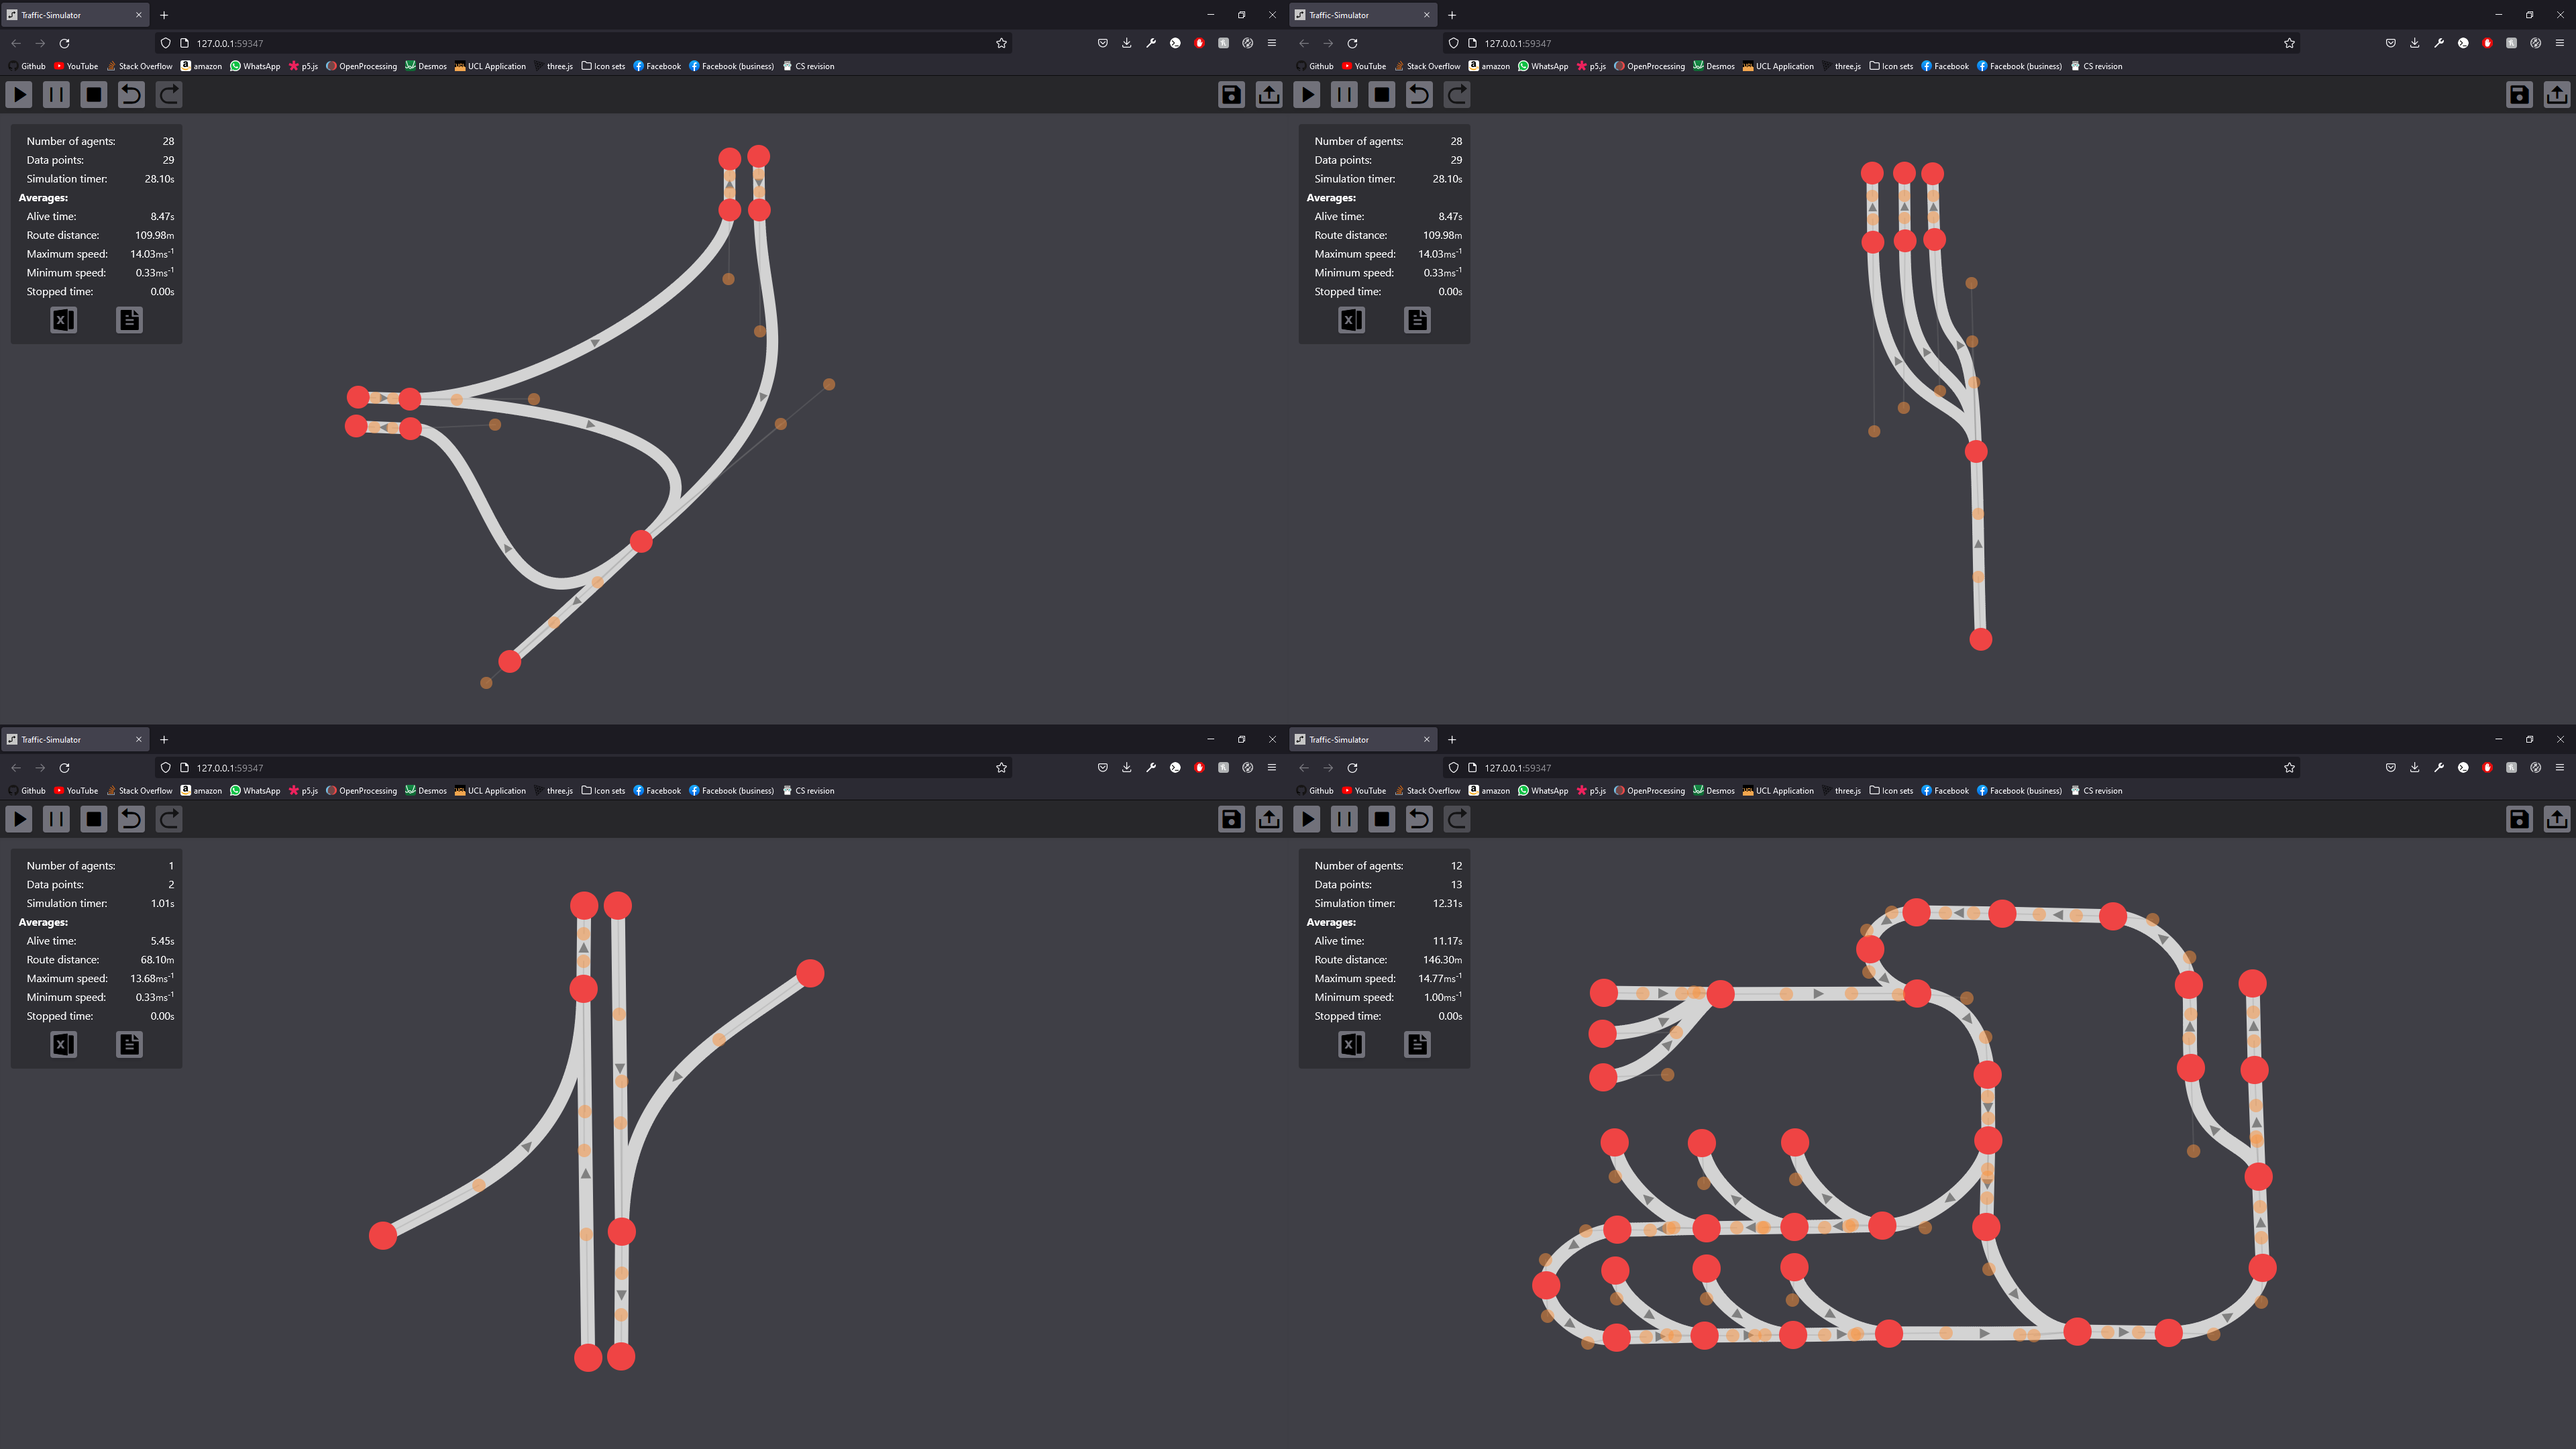
\includegraphics[width=0.8\textwidth]{example-layouts.png}
                \caption{Example road network layouts designed using my program}
                \label{testing:example-layouts}
            \end{figure}

            Shown in \autoref{testing:example-layouts} are four example layouts I constructed, all networks are rendered to the UI as expected, displaying smooth curves and everything is positioned correctly.

    \subsection{Test 2 - Vertex limit}
    \label{testing:t2}

        \subsubsection{Methodology}

            For this test I will record a video of me using the program, I will continually create new vertices until the limit is reached. Also testing the different ways of creating new vertices to ensure that there is no way for a user to surpass the limit.

            I will also add an input overlay to the video, allowing the viewer to see the inputs I have made in real time.

        \subsubsection{Results}

            The recorded video can be found at \href{https://youtu.be/03z-9HgNAaQ}{https://youtu.be/03z-9HgNAaQ}. The test ran as expected and the user was not able to create new vertices after the limit of 50 was reached. New connections that would have usually created a new vertex also behaved correctly when 50 vertices were already present.

    \subsection{Test 3 - Save and Load}
    \label{testing:t3}

        \subsubsection{Methodology}

            \begin{enumerate}
                \item Start up the program
                \item Make a simple edit to the road network
                \item Take a screenshot of the edited network
                \item Use the save feature to save the network to a local file
                \item Take a screenshot of the file inside file explorer
                \item Take a screenshot of the file's contents
                \item Restart the program
                \item Use the load feature to load the saved network into the program
                \item Take a screenshot of the new program state
            \end{enumerate}

            The expected result of this test is to have the first an last screenshots show an identical road network. The file should also contain text formatted JSON data.

            \subsubsection{Results}

                \begin{figure}[ht]
                    \centering
                    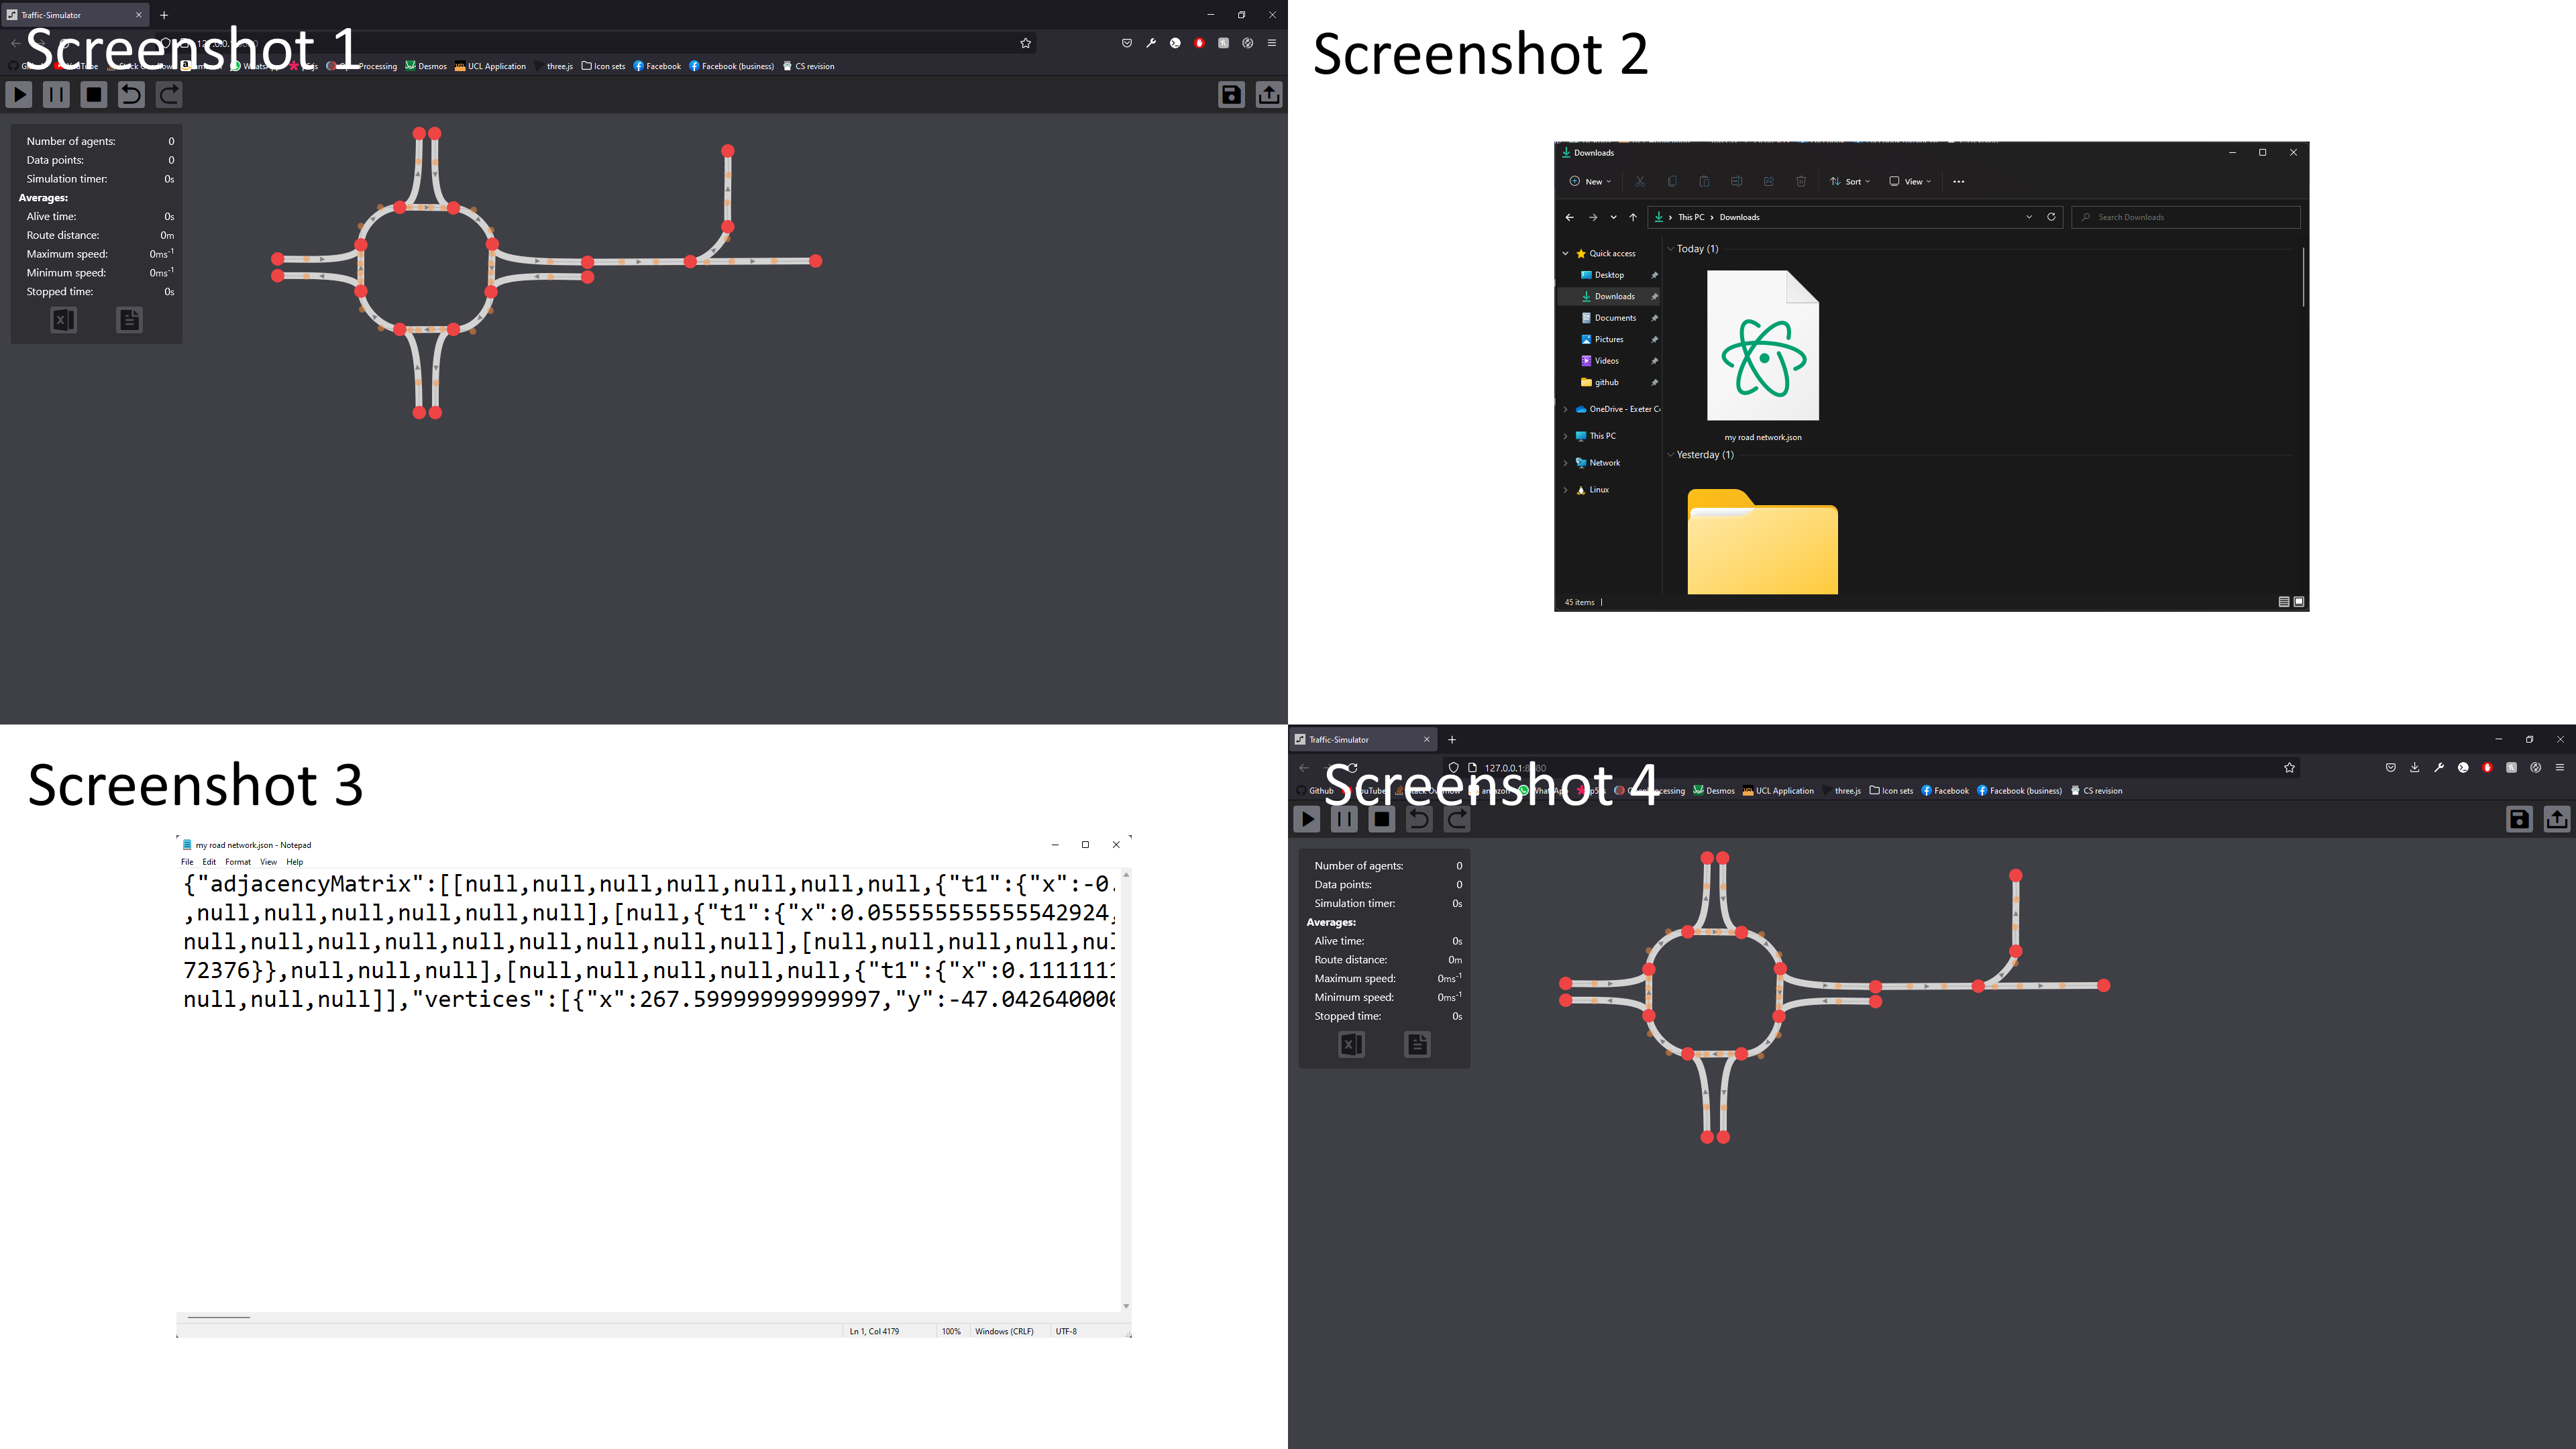
\includegraphics[width=0.8\textwidth]{t3-image.png}
                    \caption{}
                    \label{testing:t3-image}
                \end{figure}

                This test produced the expected results, Screenshot 1 shows the edited default road network. After using the save function Screenshot 2 shows a \mintTS{.json} file named \mintTS{my road network.json}. When the file is opened it shows a JSON object containing \mintTS{"adjacencyMatrix"} and \mintTS{"vertices"} attributes representing the graph data structure shown in Screenshot 3. After the load function is executed using this file Screenshot 4 was taken showing an identical layout to the inital edits.

    \subsection{Test 4 - Road network construction}
    \label{testing:t4}

        \subsubsection{Methodology}

            This test will require another video, I will start the program and use every tool provided by the program to edit the network. Theses features are as follows:

            \begin{itemize}
                \item Create new vertex
                \item Remove vertex
                \item Create new road
                \item Change road direction
                \item Remove road
                \item Create road to new vertex
                \item Reposition vertex
                \item Reposition road control point
            \end{itemize}

        \subsubsection{Results}

            \href{https://youtu.be/2Kl5lxrjS\_o}{https://youtu.be/2Kl5lxrjS\_o}. As shown in the video the user is able to perform all of the above actions without issue and the relevant alterations are seen in the network visualisation.

    \subsection{Test 5 - Undo and Redo}
    \label{testing:t5}

        \subsubsection{Methodology}

            \begin{enumerate}
                \item Start up the program
                \item Take a screenshot of the program state
                \item Make 2 simple edits to the road network
                \item Take another screenshot
                \item Use the undo feature to undo one action
                \item Take another screenshot
                \item Use the redo feature to redo one action
                \item Take a final screenshot of the program state
            \end{enumerate}

            The expected result of this test is to have the third screenshot show a single edit made to the original road network and the fourth to show two edits.

        \subsubsection{Results}

            \begin{figure}[ht]
                \centering
                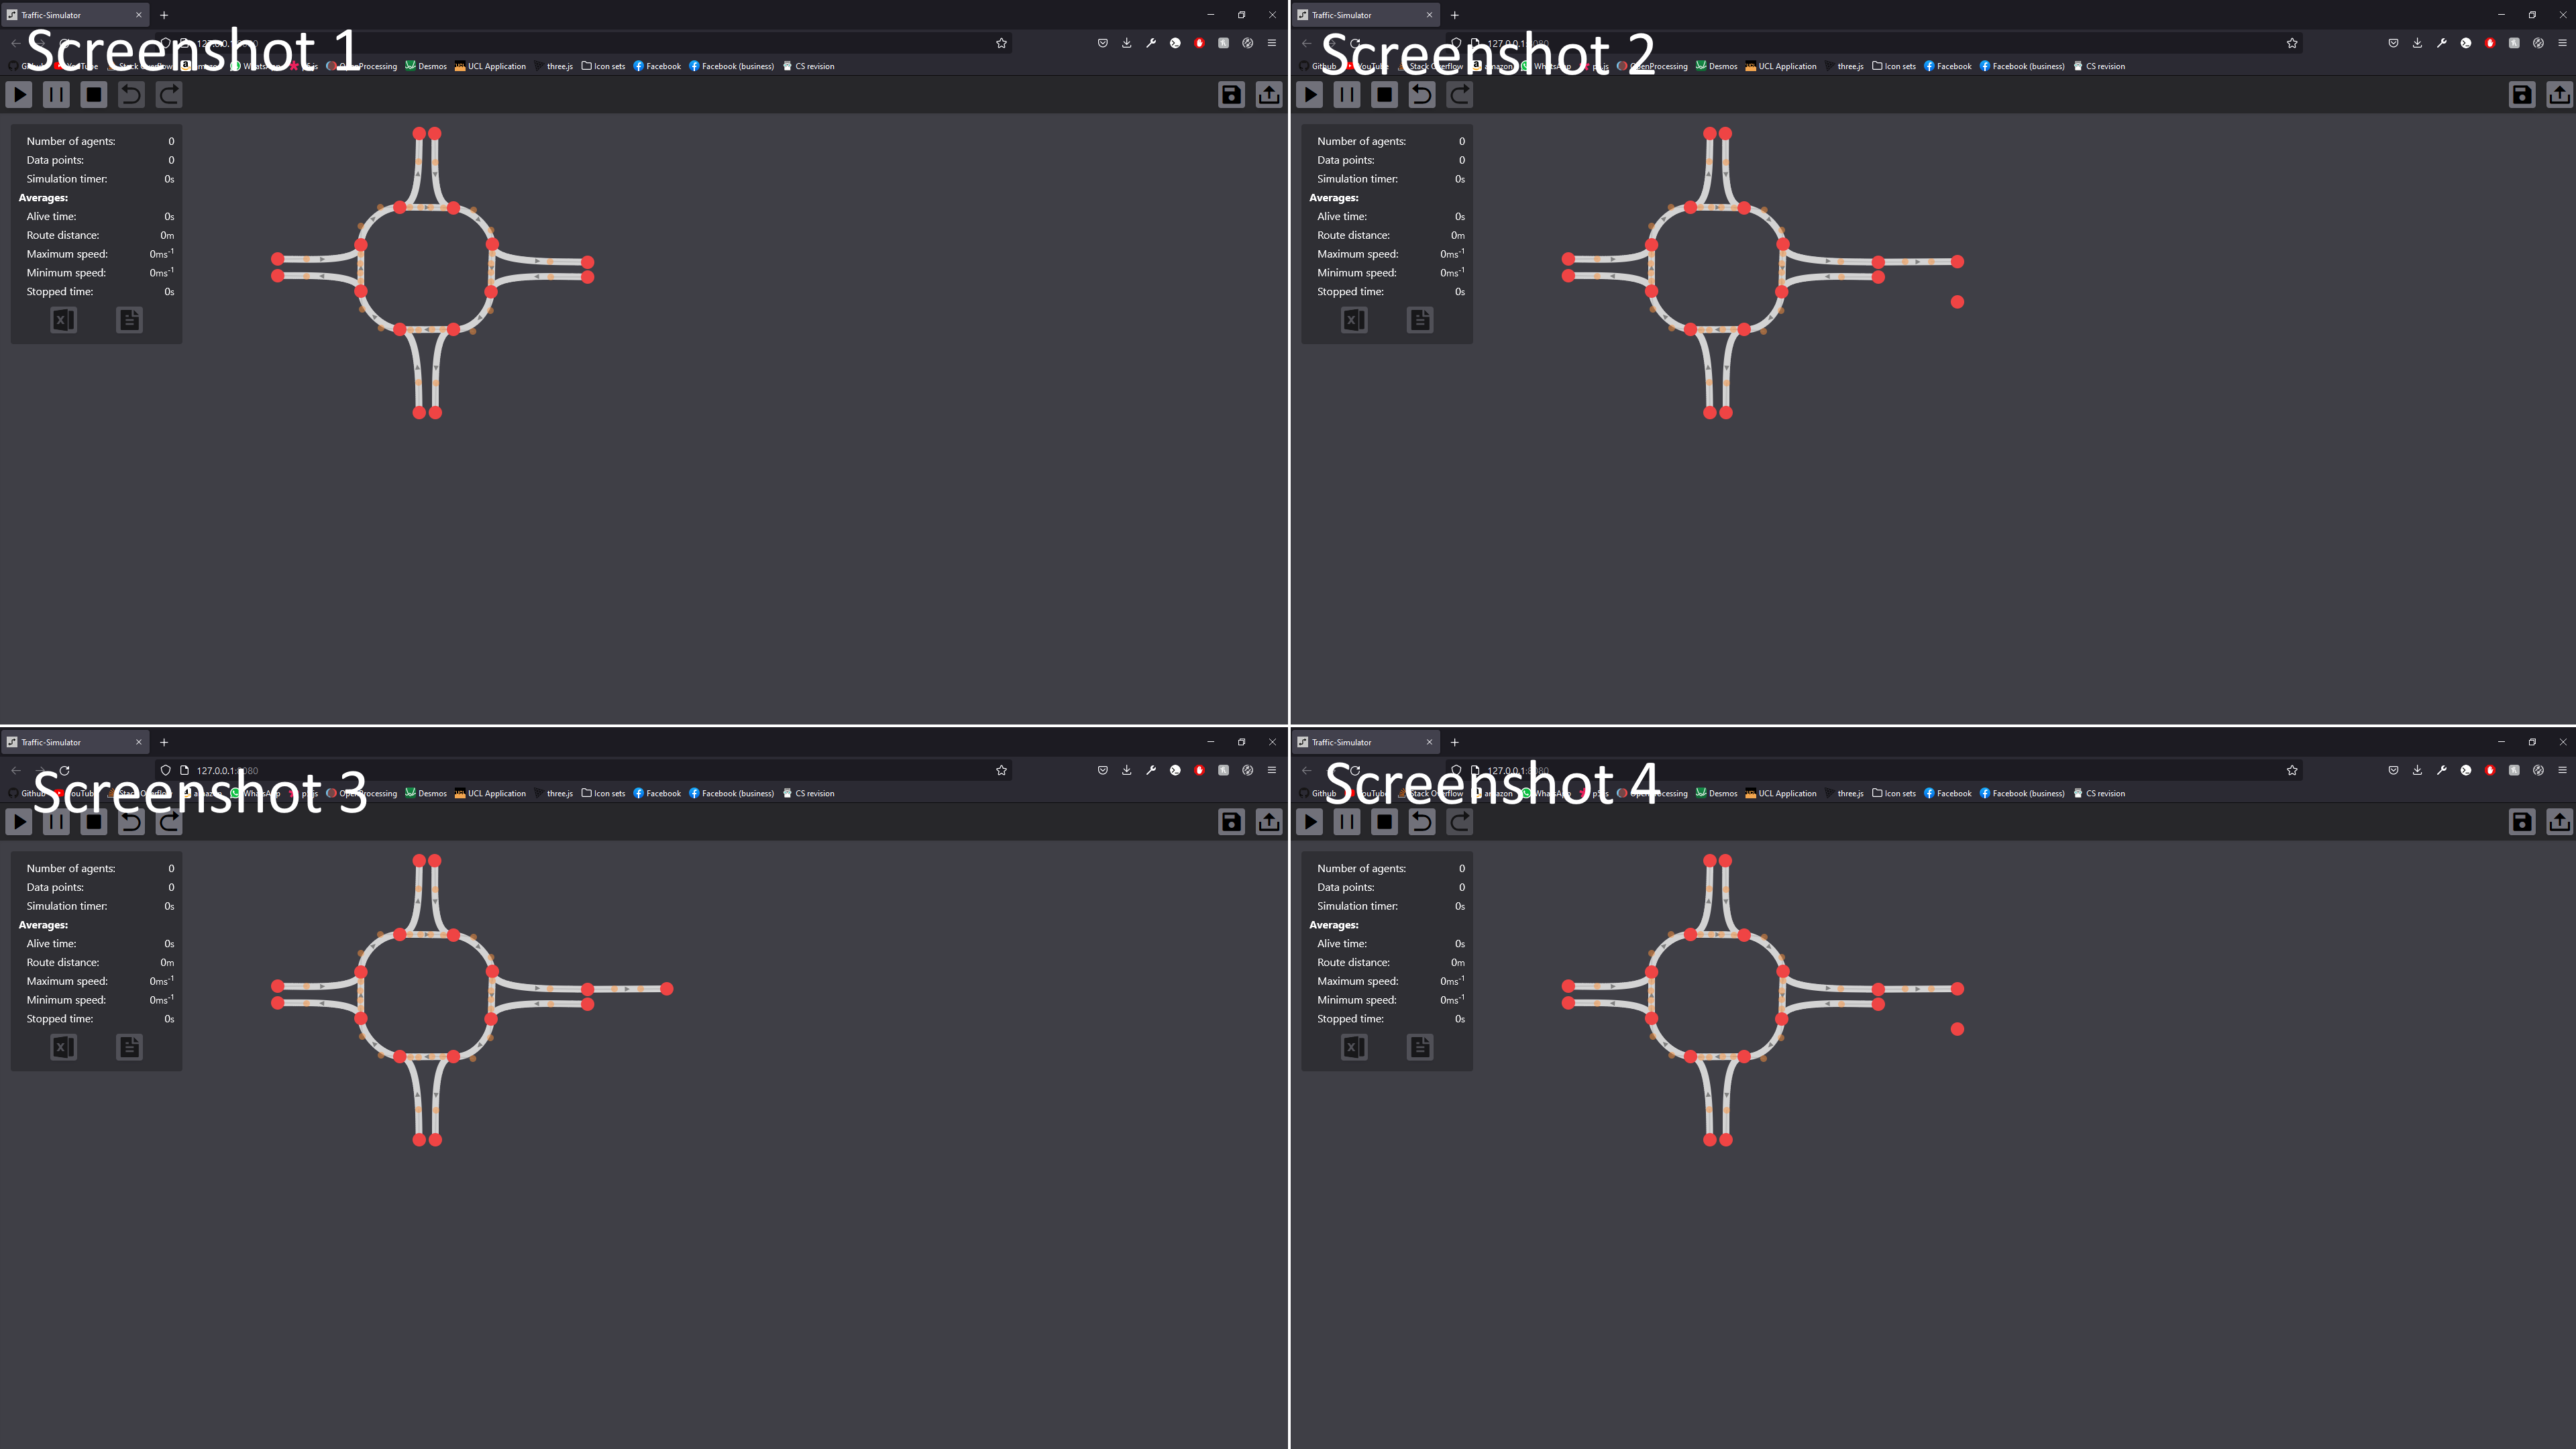
\includegraphics[width=0.8\textwidth]{t5-image.png}
                \caption{}
                \label{testing:t5-image}
            \end{figure}

            This test shows the edit of one vertex being added to the network being undone in Screenshot 3 and redone in Screenshot 4. Also visible are the 'disabled' states of the undo/redo buttons in Screenshot 1, the undo option being available after a change is made in Screenshot 2. And the redo button only becoming active after an undo operation is triggered in Screenshot 3.

    \subsection{Test 6 - Agent Movement}
    \label{testing:t6}

        \subsubsection{Methodology}

            For this test I will start the simulation using a fresh launch and making no changes to the default road network. I will capture a video of the agents moving over an arbitrary 30 second time period.

        \subsubsection{Results}

            \href{https://youtu.be/pmxqU6VuwSY}{https://youtu.be/pmxqU6VuwSY}. This test successfully demonstrates a few behaviours of the agents:

            \begin{itemize}
                \item Agents accelerate from rest once and stop accelerating once some maximum road velocity is reached.
                \item Agents will slow down or stop when another agent is detected travelling in a similar direction. The emergent behaviour of this causes agents to 'give way' to one another when approaching junctions.
                \item Agents successfully follow their generated routes, starting from a source vertex and travelling along valid paths (respecting the directions of edges) to a connected exit vertex.
            \end{itemize}

    \subsection{Test 7 - Maximum agent limit}
    \label{testing:t7}

        \subsubsection{Methodology}

            Admittedly this feature is a little harder to test, for this test I will need to construct a rather large network, capable of holding 60 agents. I will then run the simulation and wait for 60 agents to spawn and be concurrently active in the network, when I think this point has been reached and the number of agents is no longer increasing I will take a few screenshots of the program, I will then count the number of agents on screen and verify that this number does not exceed 60.

        \subsubsection{Results}

            \textbf{INSERT IMAGE HERE}

    \subsection{Test 8 - Data Output}
    \label{testing:t8}

        \subsubsection{Methodology}

            This test will validate the programs ability to provide output data to the user, using the following procedure.

            \begin{enumerate}
                \item Start up the program
                \item Start the simulation using the default road network
                \item Let the student run for a sufficient length of time, roughly 40 data points
                \item Pause the simulation and take a screenshot of the current program state
                \item Use the save output data feature to export a \mintTS{.xlsx} and \mintTS{.csv} file
                \item Take screenshots of the files in file explorer
                \item Open both files and screenshot their contents
            \end{enumerate}

            I expect the number of samples present in the output files to match the number of samples shown on screen, as well as having reasonable values given the summary data.

        \subsubsection{Results}

            \begin{figure}[ht]
                \centering
                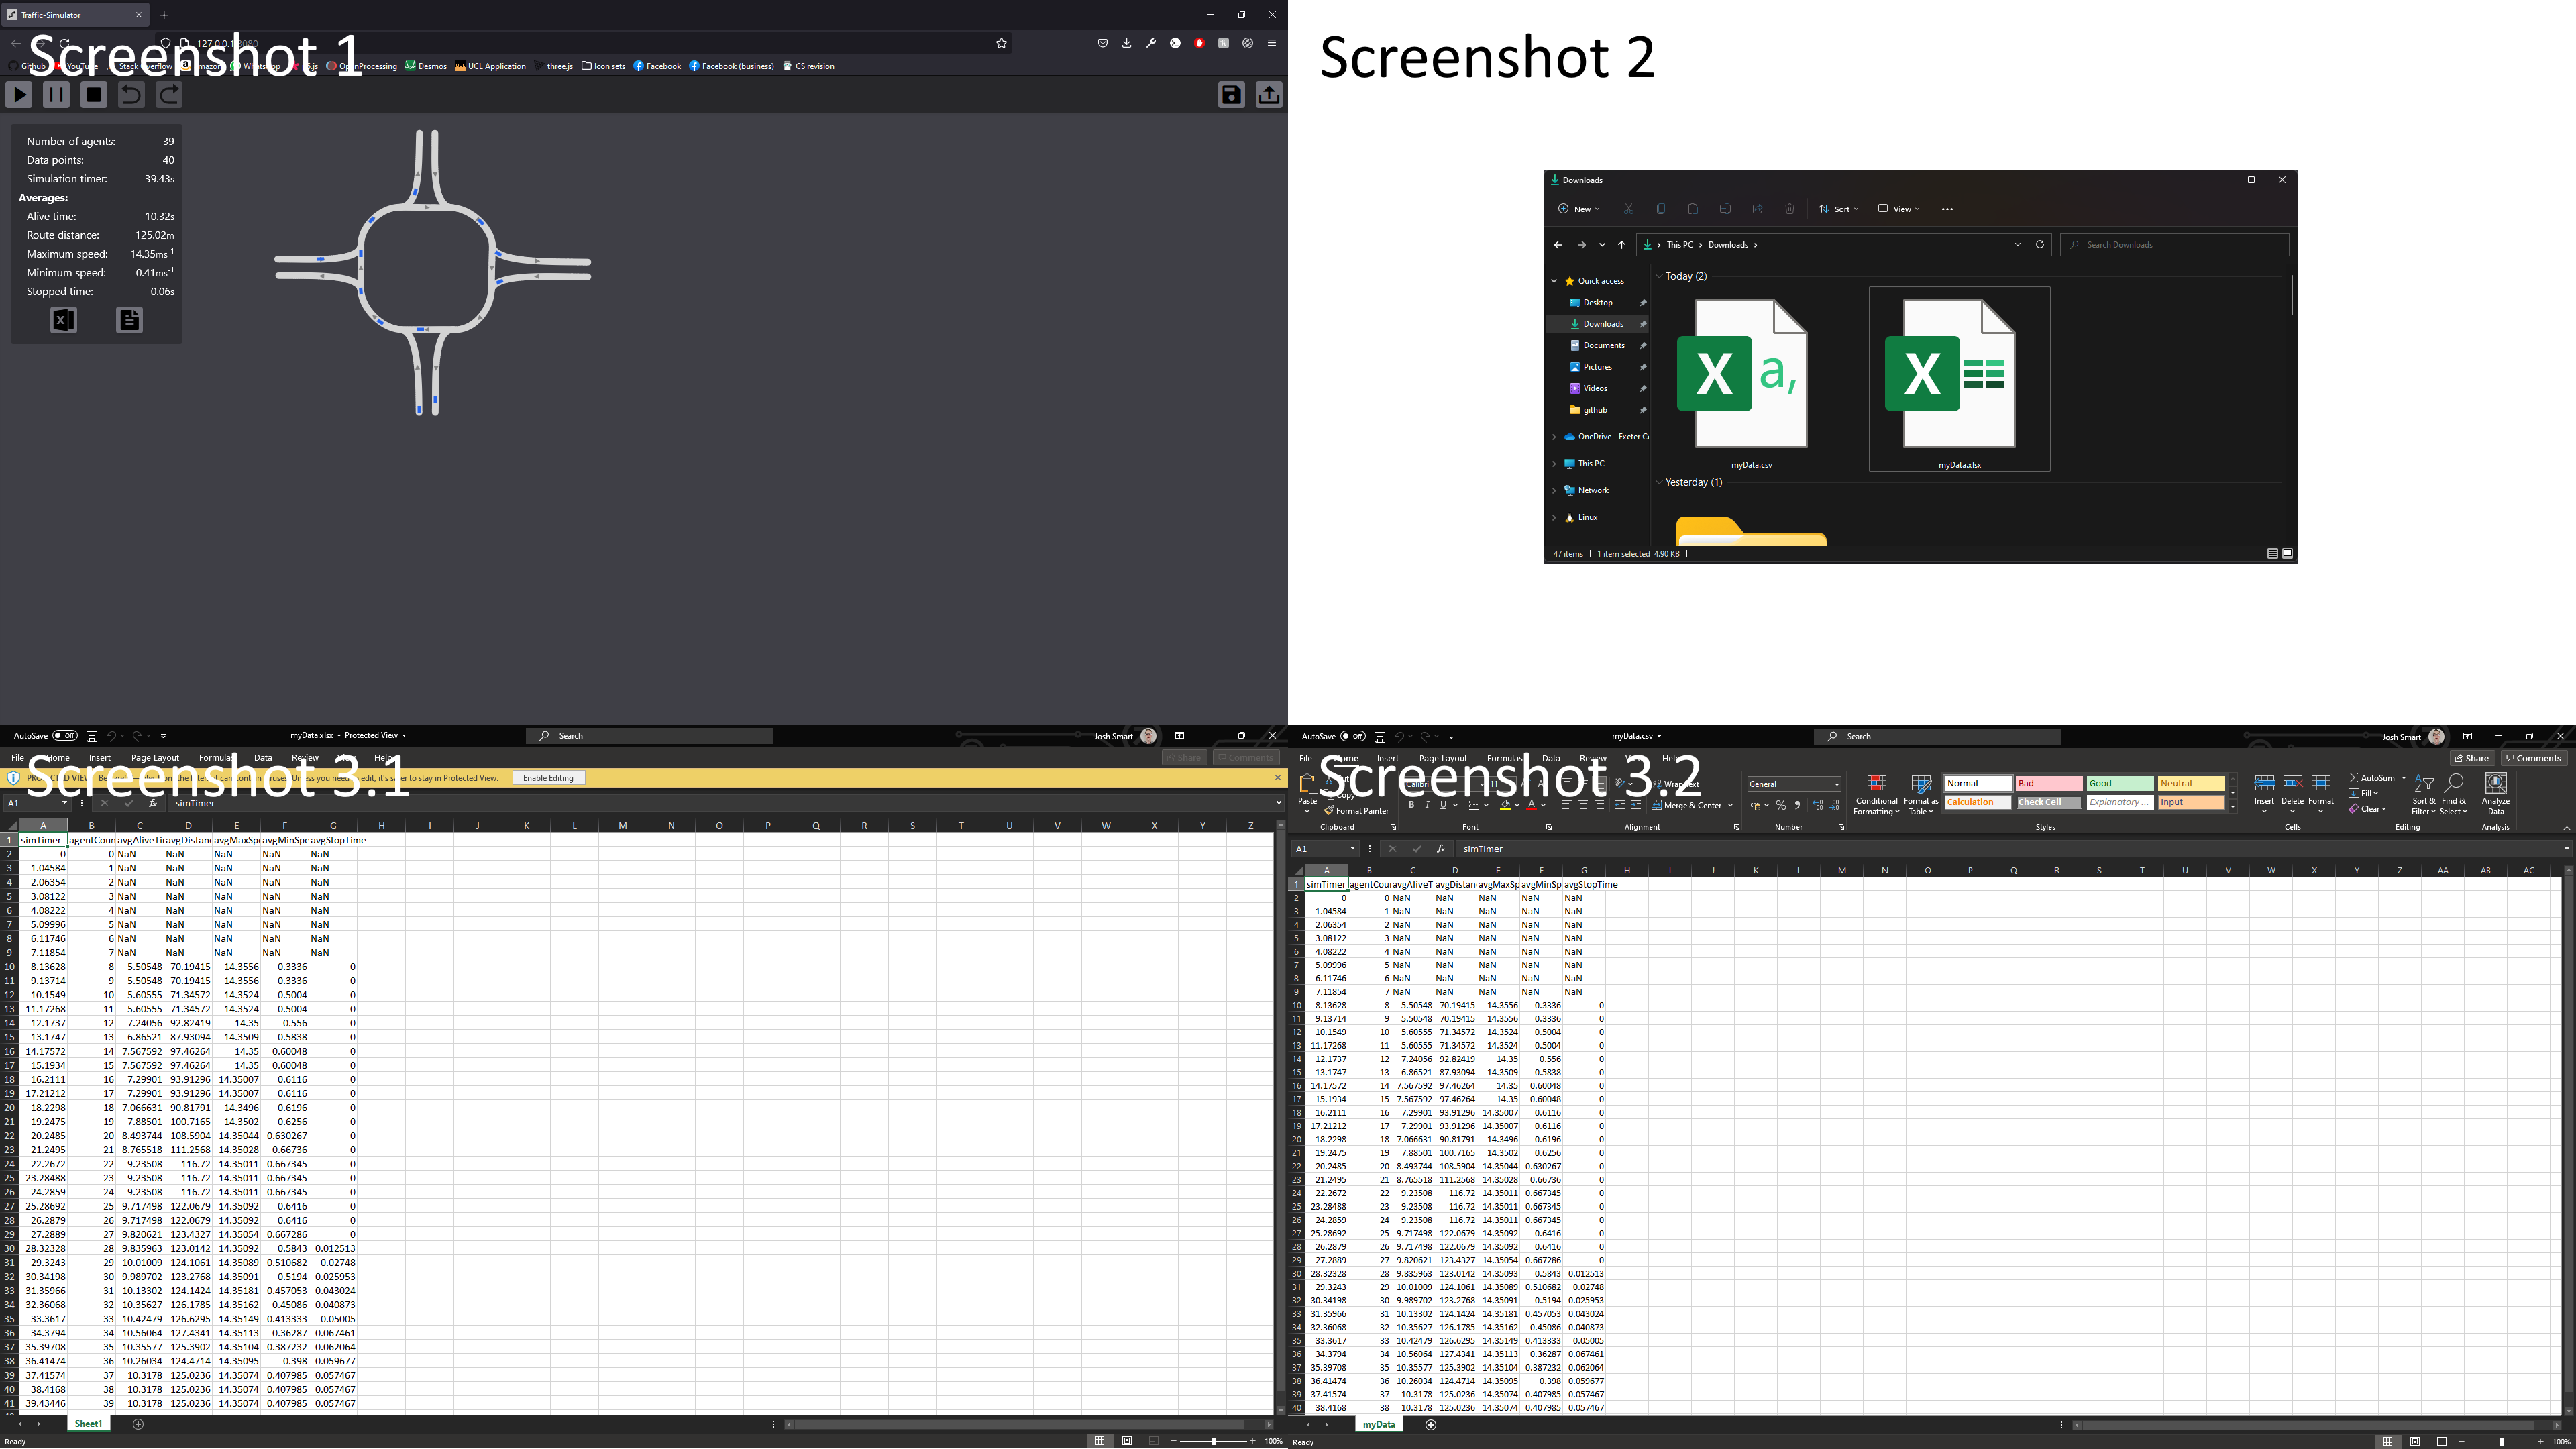
\includegraphics[width=0.8\textwidth]{t8-image.png}
                \caption{}
                \label{testing:t8-image}
            \end{figure}

            Screenshot 1 shows the summary output data display, indicating 40 data points have been collected. After using the save data output function, Screenshot 2 shows two files named \mintTS{myData.xlsx} and \mintTS{myData.csv}. Viewing the contents of these files gives Screenshots 3.1 and 3.2, as expected both these files contain an identical 40 rows of information. The leading rows of \mintTS{NaN} are expected behaviour as this represents the frames in which no agents had concluded their route so no data is present.

    \subsection{Tests 9, 10, 11 - GUI Compatibility}
    \label{testing:t9,10,11}

        \subsubsection{Methodology}

            To address the last 3 requirements in my summary, I will use my browser's inbuilt dev tools to test to programs behaviour on a series of different sizes and aspect ratios, capturing screenshots as I go. I expect the UI to resize elements in order to fit the screen size it has been given.

        \subsubsection{Results}

            \textbf{INSERT IMAGES}

\section{Back-end}

    During the development process I wrote a series of unit tests to validate the major parts of the system, leading to less error-prone and maintainable code. The following index (\autoref{tests-index}) points to the test files in my code base. All the tests pass when executed.

    \begin{table}[ht]
        \begin{tabular}{|p{0.45\textwidth}|p{0.45\textwidth}|}
            \hline
            \textbf{Test target} & \textbf{Link}\\\hline
            Graph & \href{https://github.com/joshua-smart/traffic-simulator/blob/main/src/tests/model/graph.test.ts}{src/tests/model/graph.test.ts}\\\hline
            RoadNetwork & \href{https://github.com/joshua-smart/traffic-simulator/blob/main/src/tests/model/roadNetwork.test.ts}{src/tests/model/roadNetwork.test.ts}\\\hline
            Simulation & \href{https://github.com/joshua-smart/traffic-simulator/blob/main/src/tests/model/simulation.test.ts}{src/tests/model/simulation.test.ts}\\\hline
        \end{tabular}
        \caption{Unit tests index}
        \label{tests-index}
    \end{table}
